\chapter{Approach}
The author in \cite{b6} proposes a step approach to carry out desynchronization attacks. Figure \ref{fig:Phases} shows the phases of a desynchronization attack or request smuggling. Before explaining each of the phases in request smuggling, we need to observe that there are four possible configurations between the systems:
\begin{itemize}
	\item \textbf{CL.CL : } Both the frontend and backend servers use \textsc{Content-Length} header. As we have already seen, this configuration doesn't help in realizing attacks on practical modern systems. 
	\item \textbf{CL.TE : } Frontend server uses \textsc{Content-Length} header field and Backend server uses \textsc{Transfer-Encoding} header field. 
	\item \textbf{TE.CL : } Frontend server uses \textsc{Transfer-Encoding} header field and Backend server uses \textsc{Content-Length} header field.
	\item \textbf{TE.TE : } Both the frontend and backend servers use \textsc{Transfer-Encoding} header field.
\end{itemize}
\begin{figure}
	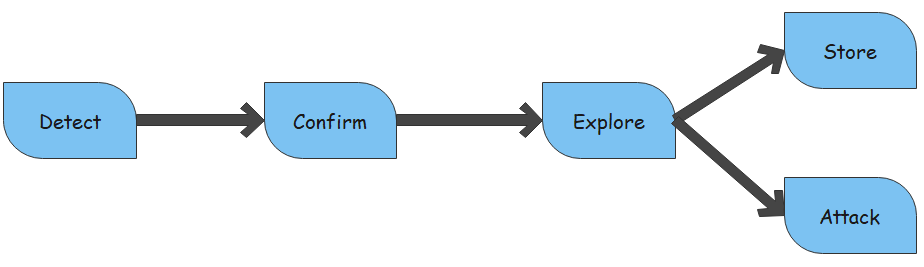
\includegraphics[width=14cm]{images/Phases}
	\caption{Phases of request smuggling}
	\label{fig:Phases}
\end{figure}
We will now look at each of the phases in detail:
\section{Detect}
The first step is to detect when a server will be vulnerable to desynchronization.  
\section{Confirm}
\section{Explore}
\section{Store}
\section{Attack}